\section*{Схема экспериментальной установки}

Схема установки изображена на рисунке:

\begin{figure}[H]
	\centering
	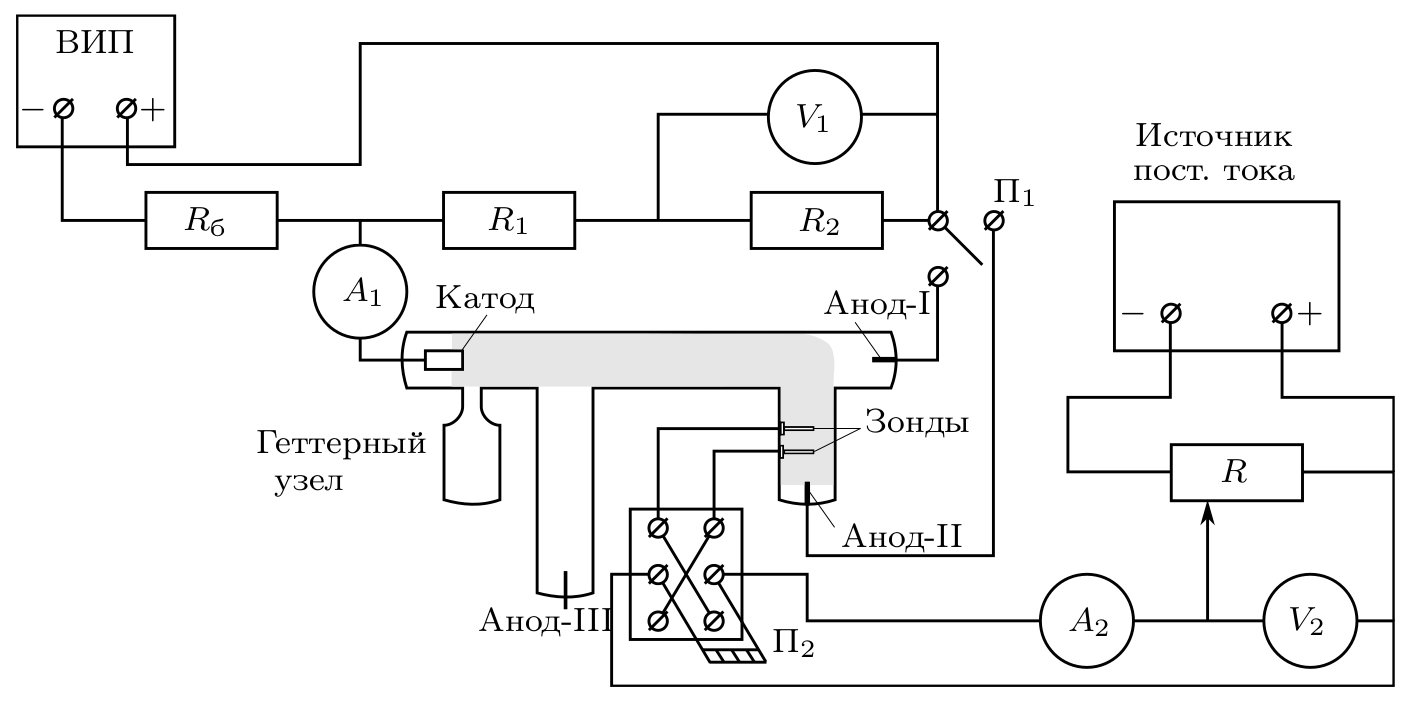
\includegraphics[width=1\textwidth]{../res/exp scheme.png}
\end{figure}

Стеклянная газоразрядная трубка имеет холодный (нагреваемый) полый катод, три анода и геттерный узел --- стеклянный баллон, на внутреннюю поверхность которого напылена газопоглощающая плёнка. Трубка наполнена изотопом неона $^{22}Ne$ при давлении 2 мм рт. ст. Катод и один из анодов ($I$ или $II$) с помощью переключателя $П_1$ подключается через балластный резистор $R_б (\sim 450 кОм)$ к регулируемому высоковольтному источнику питания (ВИП) с выходом напряжением до 5 кВ. 